\documentclass[conference]{IEEEtran}
\usepackage{graphicx}
\usepackage{amsmath}
\usepackage{cite}
\usepackage{float} 
\usepackage{url} 

\title{A Technical Report on Wireless Site Survey and Architecture of Roaming for Wireless Access Networks in Commercial Areas.}

\author{
    Pham Xuan Bach, Nguyen Duc Chi Dat, and Nguyen Khanh Toan\\
    \textit{Faculty of Computing, Engineering and the Built Environment } \\
    \textit{University of Information Technology} \\
    Ho Chi Minh City, Vienam \\
    \{bachpx.19, datndc.19, toannk.19\}@grad.uit.edu.vn
}


\begin{document}

\maketitle

\begin{abstract}
This report investigates Wi-Fi coverage and signal strength at a specific area in GigaMall Shopping Center, Thu Duc, and explains the basic architecture of the network's roaming currently in use.
\end{abstract}

\begin{IEEEkeywords}
wireless site survey, roaming architecture, coverage analysis
\end{IEEEkeywords}

\section{Introduction}

Wireless site surveys are useful for ensuring good performance and coverage of Wi-Fi networks in equipped environments, especially in locations like shopping centers, as they require a stable Wi-Fi connection for a large number of users. Surveys should be conducted in small areas for more accuracy. This report aims to present findings and assess Wi-Fi signal strength, and coverage areas on the first floor of GigaMall Shopping Center, Thu Duc. These findings and assessments will serve as a basis for recommendations to enhance the network. Additionally, the report will explain the roaming architecture implemented to optimise connectivity across different areas within the network and improve overall user experience.

\section{Wireless Site Surveys}

\subsection{Site Description}

This area is the GigaMall Shopping Center in Thu Duc, frequently visited by local residents due to its many shopping and entertainment zones, as well as large supermarket systems. The surveyed floor is the first floor, covering an area of approximately 12,000 square meters. The layout consists of shops, stairs, and corridors. The walls are made of plastic partitions with a steel frame, and the doors are made of glass.

The survey was conducted on the weekend during peak hours. The highest density was recorded at Highland Coffee, where a large number of people gathered to relax.

\subsection{Methodology}

To ensure a thorough assessment of network conditions, a strategic selection of survey points was made. These points were carefully chosen to provide representative coverage across the entire mall, encompassing various areas such as common spaces, retail outlets, and food courts. A floor map was generated using data from the official GigaMall website. Network access points were identified and marked on the map. The next steps involved identifying the points to be surveyed; these selected points had to be specific locations to ensure that the survey covered nearly all aspects of the floor. To facilitate data collection, specialized network measurement tools were configured on mobile and laptop devices. 

Specifically, \textit{speedtest-cli} utility is used to quantify internet performance metrics, including upload and download speeds as well as network latency. Due to the large number of points to be surveyed, a Python script was utilized to automate the process and save the records into a text file whenever one of these points was reached. Moreover, \textit{lswifi} commandline tool was employed to list all the recognizable Wi-Fi networks within range, capturing essential details such as Service Set Identifiers (SSIDs), Received Signal Strength Indicators (RSSIs), channels, frequencies, security protocols, and 802.11 standards. Additionally, the Wifi Heatmap application downloaded from the Google Play Store is used to survey signal strength. By walking around, signal strength was measured and the map was colored accordingly to generate a heatmap.

Given the substantial number of survey points, a Python script was developed to automate the data collection process. This script enabled the efficient recording of network measurements at each designated location, storing the results in a csv file for subsequent analysis.

Once preparations were complete, the next step was to walk through the marked locations and capture the necessary information. It was important to note the points where the device could switch from one access point to another. The collected data will be visualized using Microsoft Excel and Chart.js to generate graphical representations. The resulting visualizations will be presented in the subsequent section.

\subsection{Findings and Analysis}

Fig. 1 below is the heatmap illustrating the Wi-Fi signal strength received by the device across the floor, with four access points located at positions as shown on the map. Signal strength is visually represented by a color gradient, ranging from red (strongest signal) to orange, yellow, and blue (weakest signal).

\begin{figure}[htbp]
    \centering
    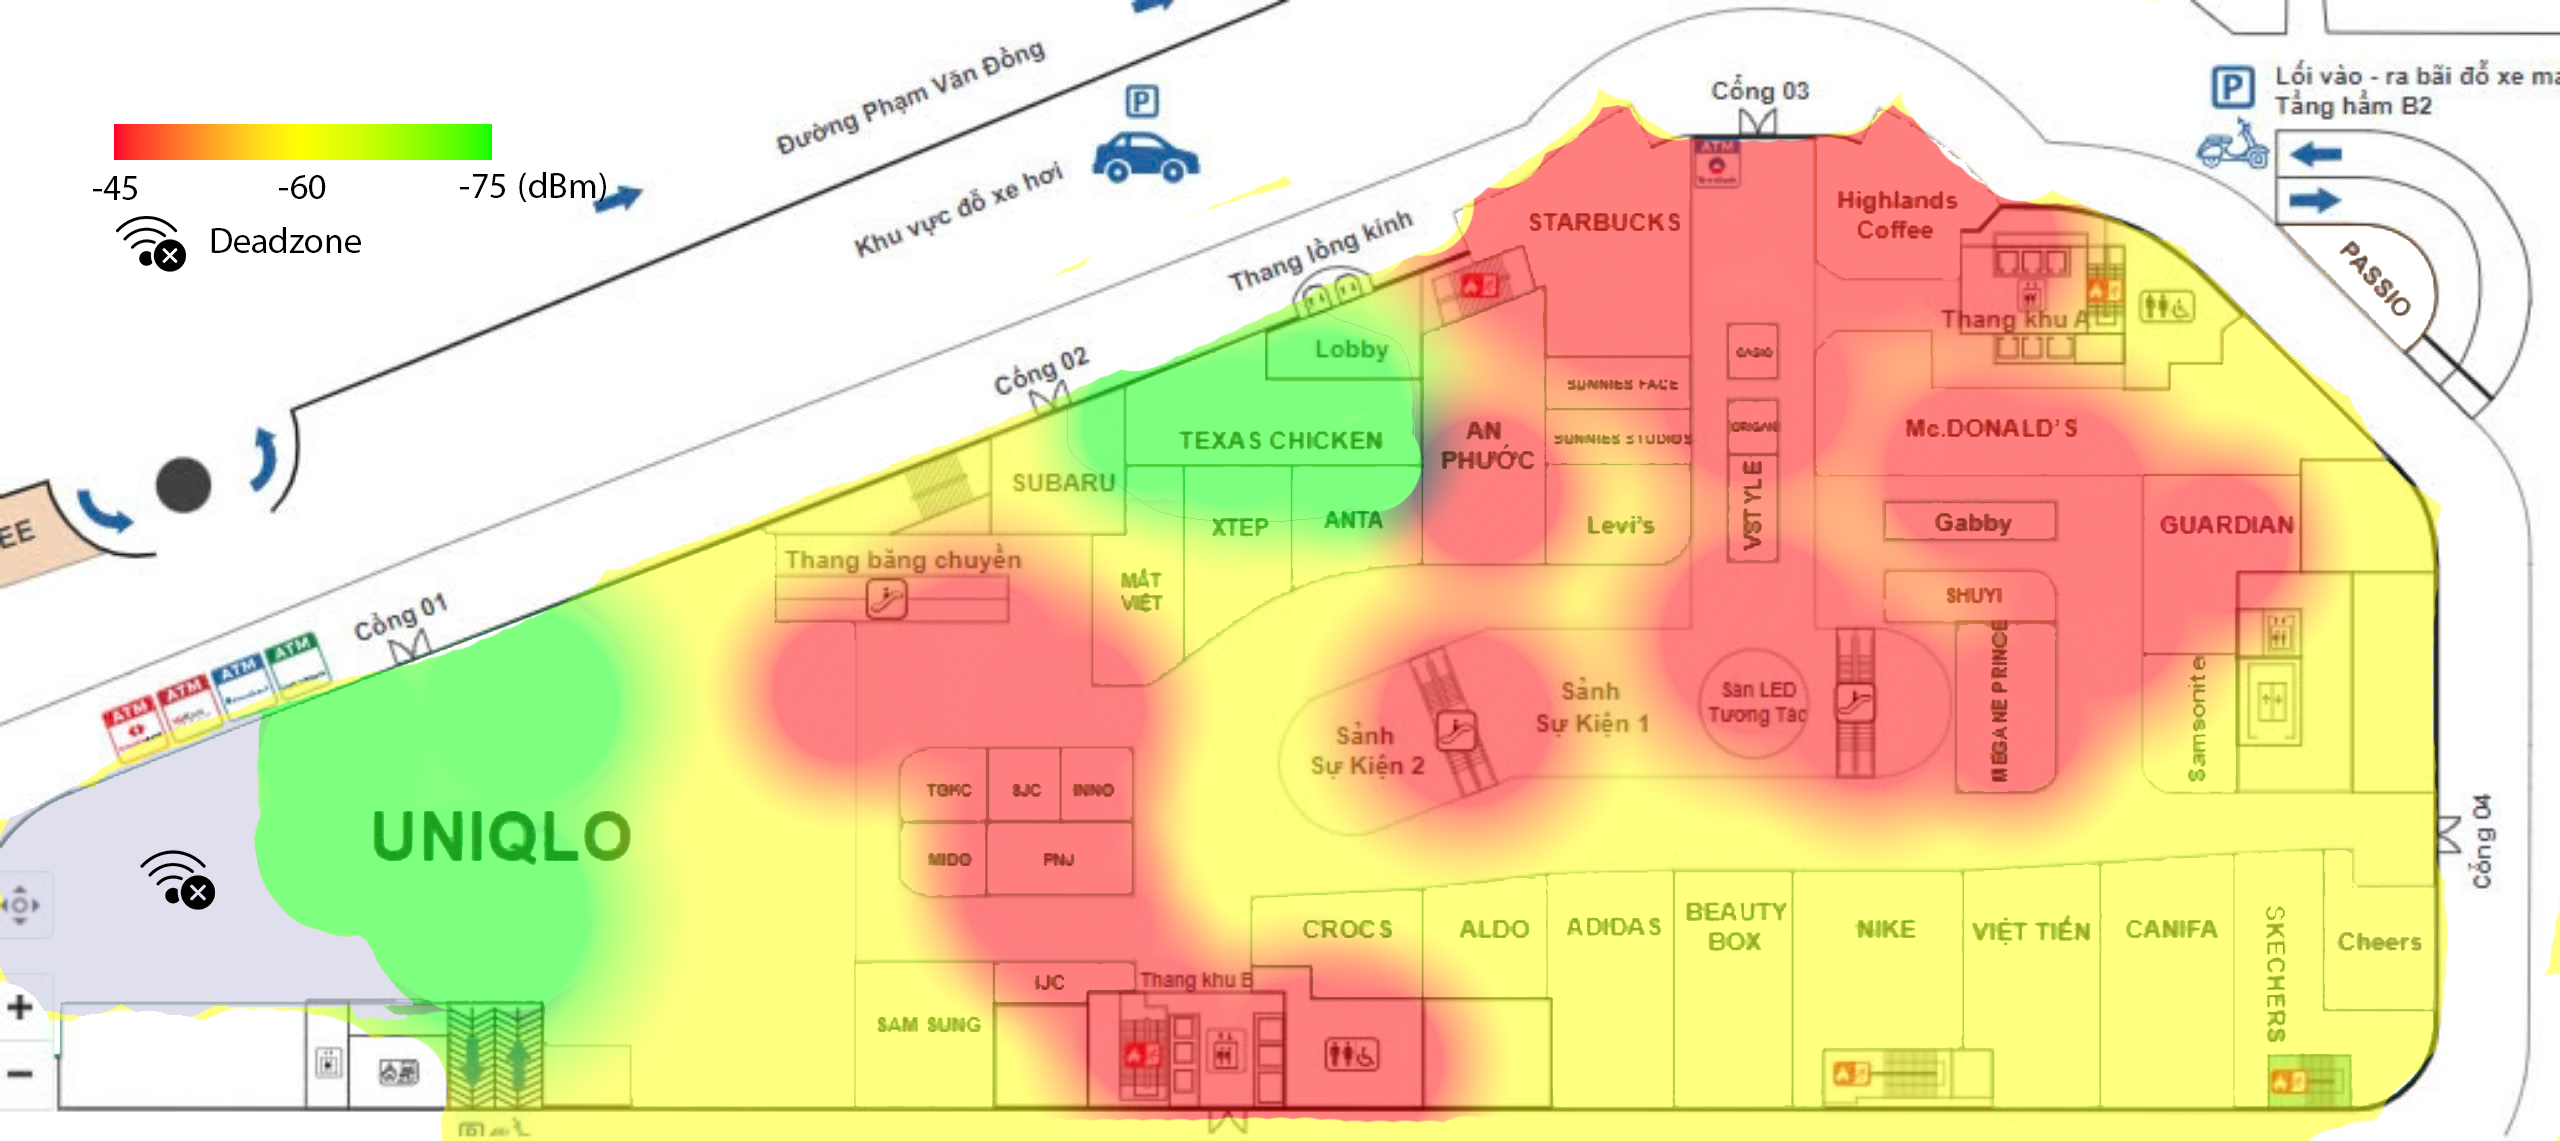
\includegraphics[width=0.48\textwidth]{fig1_heatmap.png}
    \caption{Heatmap of Wi-Fi signal coverage on the first floor of GigaMall Shopping Center.}
\end{figure}

The spacious central area on the map is a common space within the shopping mall, equipped with approximately 4 public Wi-Fi access points to meet the high demand of visitors for browsing, online shopping, and entertainment. As can be seen from the map, the signal in this area is always measured below -60 dBm, which was only sufficient at the time the survey was conducted. Within a 10-meter radius of each access point, a level above -60 dBm can be achieved. However, the stability is not high due to the large number of connections accessing simultaneously. Improving the signal strength would be beneficial to ensure more reliable and faster connections, especially during peak usage periods.

The surrounding areas are shop houses separated from the common space by walls, glass, and large plastic panels. Despite being within the shopping center, these shop houses suffer from poor Wi-Fi signal strength. Consequently, most shop houses have deployed their own Wi-Fi networks, leading to a dense Wi-Fi environment. This high density of Wi-Fi networks can result in interference, particularly when multiple networks operate on the same channel or frequency band (2.4GHz or 5GHz). As illustrated in Fig 2, signal strength typically decreases with distance from the access point, but factors such as physical obstructions, high density of Wi-Fi networks and a large number of concurrent connections can cause deviations from this general trend, resulting in non-monotonic chart values.

\begin{figure}[htbp]
    \centering
    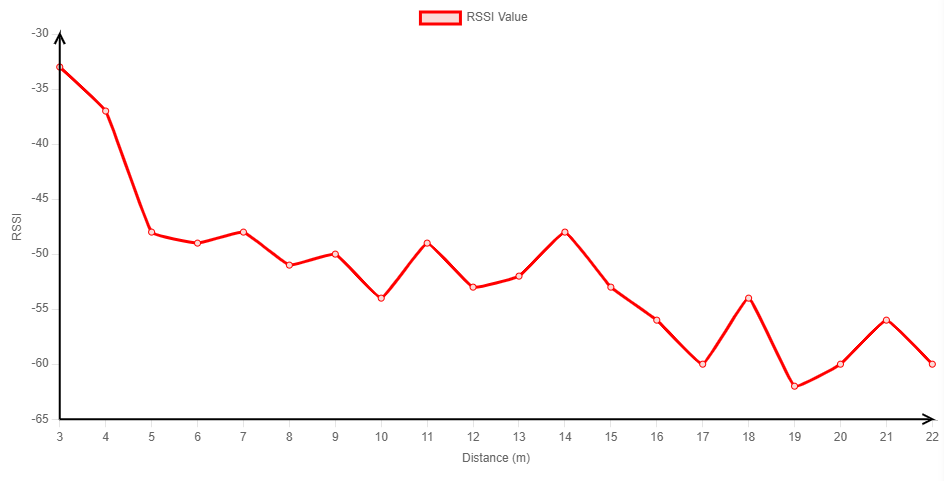
\includegraphics[width=0.48\textwidth]{fig2_rssi.png}
    \caption{A line chart shows the relationship between distance from access point and RSSI.}
\end{figure}

Fig. 3 compares the signal strength under line-of-sight (LoS) and non-line of sight (Non-LoS) conditions. Signal strength measurements were collected over a 120-second interval while connected to the same access point at a fixed distance. As shown, the LoS condition consistently exhibits stronger signal strength and less attenuation compared to the Non-LoS condition.

\begin{figure}[htbp]
    \centering
    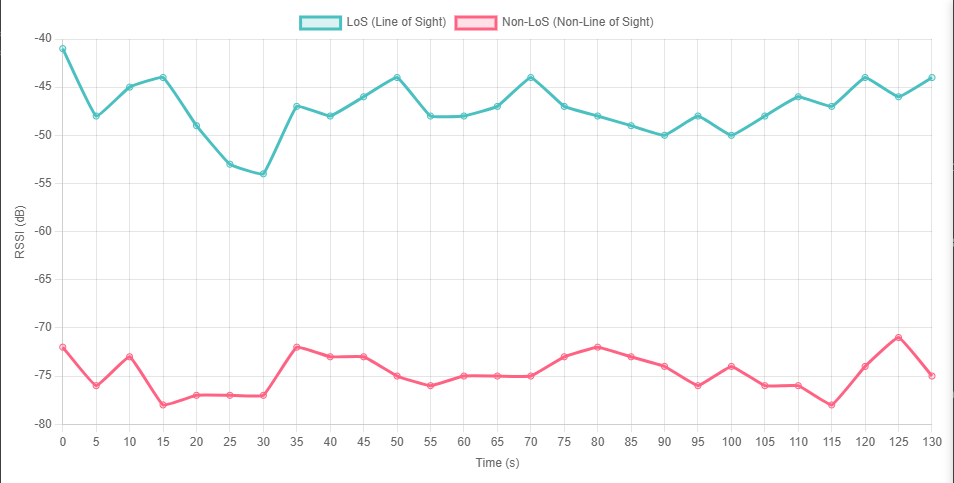
\includegraphics[width=0.48\textwidth]{fig3_los_nonlos.png}
    \caption{A graph illustrates signal strength in LoS and Non-LoS conditions.}
    \label{fig:los_nonlos}
\end{figure}

Additionally, data on upload and download speeds, as well as latency at each surveyed spot, are illustrated in Fig. 4. The green line represents latency in milliseconds (ms) on the right axis, while the red and blue bars represent upload and download speeds in Megabits per second (Mbps) respectively.

\begin{figure}[htbp]
    \centering
    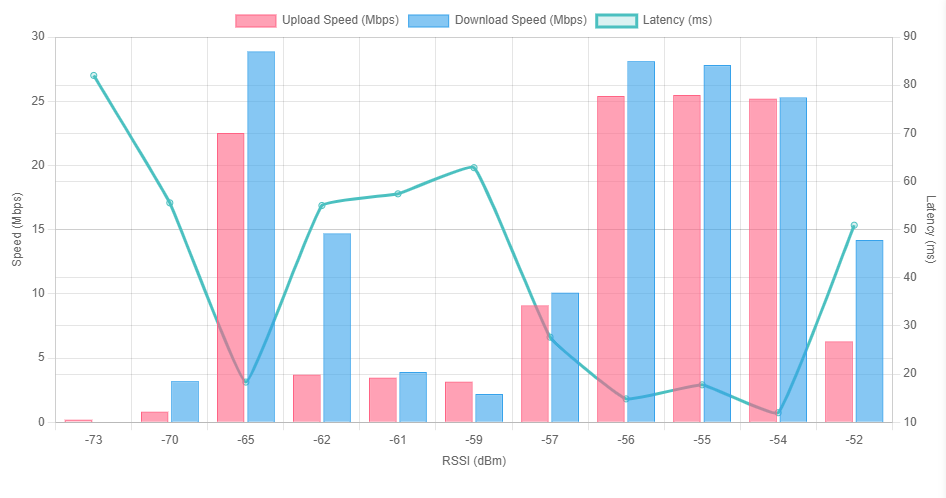
\includegraphics[width=0.5\textwidth]{fig4_speed_test.png}
    \caption{Relationship between RSSI and Network Performance.}
\end{figure}

The green line, representing latency, demonstrates an inverse correlation with RSSI. As signal strength (RSSI) diminishes, latency increases, and conversely. For instance, at low RSSI values (approximately -73 dBm), latency is elevated (above 70 ms), indicating a direct relationship between weak signal strength and increased data transmission delays. High latency potentially affects real-time applications like online gaming or video streaming.

As signal strength improves (higher RSSI values), both upload and download speeds increase. The peak upload and download speeds are achieved at RSSI values between -56 dBm and -54 dBm, with download speeds exceeding 25 Mbps and upload speeds reaching approximately 20 Mbps. Conversely, at weaker signal levels (e.g., -73 dBm), speeds are significantly reduced, approaching negligible levels. 

A clear correlation exists between stronger Wi-Fi signals (higher RSSI) and improved network performance, encompassing faster upload/download speeds and lower latency. The chart indicates that elevating signal strength, particularly above -60 dBm, can substantially enhance both speed and user experience by reducing latency. However, there are instances where the data deviates from the expected theoretical relationship due to the inherent instability of Wi-Fi signals as described in Fig. 2. A case in point is the anomalous spike in both download and upload speeds observed at an RSSI of -65 dBm.

The survey also identified two roaming areas where the access points overlapped and the device transitioned between access points without any signal interruption. Fig. 5 displays the changes in the access point BSSID, which is the MAC address of the access point, as the device moves into the roaming areas. Nonetheless, it discovered a dead zone where the Wi-Fi connection was disconnected before connecting to a new access point, indicating that the roaming transition in this area was not as smooth as expected. The reason for that situation is that the distance between the two access points is quite large, and signal strength is insufficient so the area cannot be fully covered. The roaming architecture will be discussed in more detail in section III.

\begin{figure}[htbp]
    \centering
    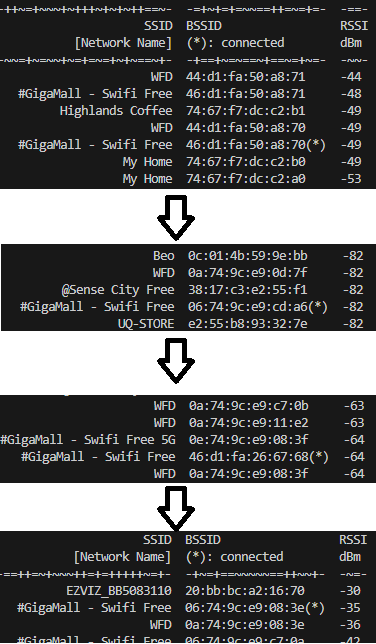
\includegraphics[width=0.44\textwidth]{fig5_rssid_change.png}
    \caption{An output demonstrates BSSID changes at each roaming spot.}
\end{figure}

\subsection{Recommendations for the network}

The site survey results suggest that optimizing the network system requires several improvements. Specifically, the placement of access points should be optimized, and more access points should be deployed in areas prone to interference. To address the low-signal areas on the first floor of the shopping mall, this study proposes installing three additional access points to mitigate dead zones in these areas and improve signal coverage for seamless roaming. This will also help distribute the network load, alleviating congestion. The recommended locations for the new access points are illustrated in Fig. 6.

\begin{figure}[htbp]
    \centering
    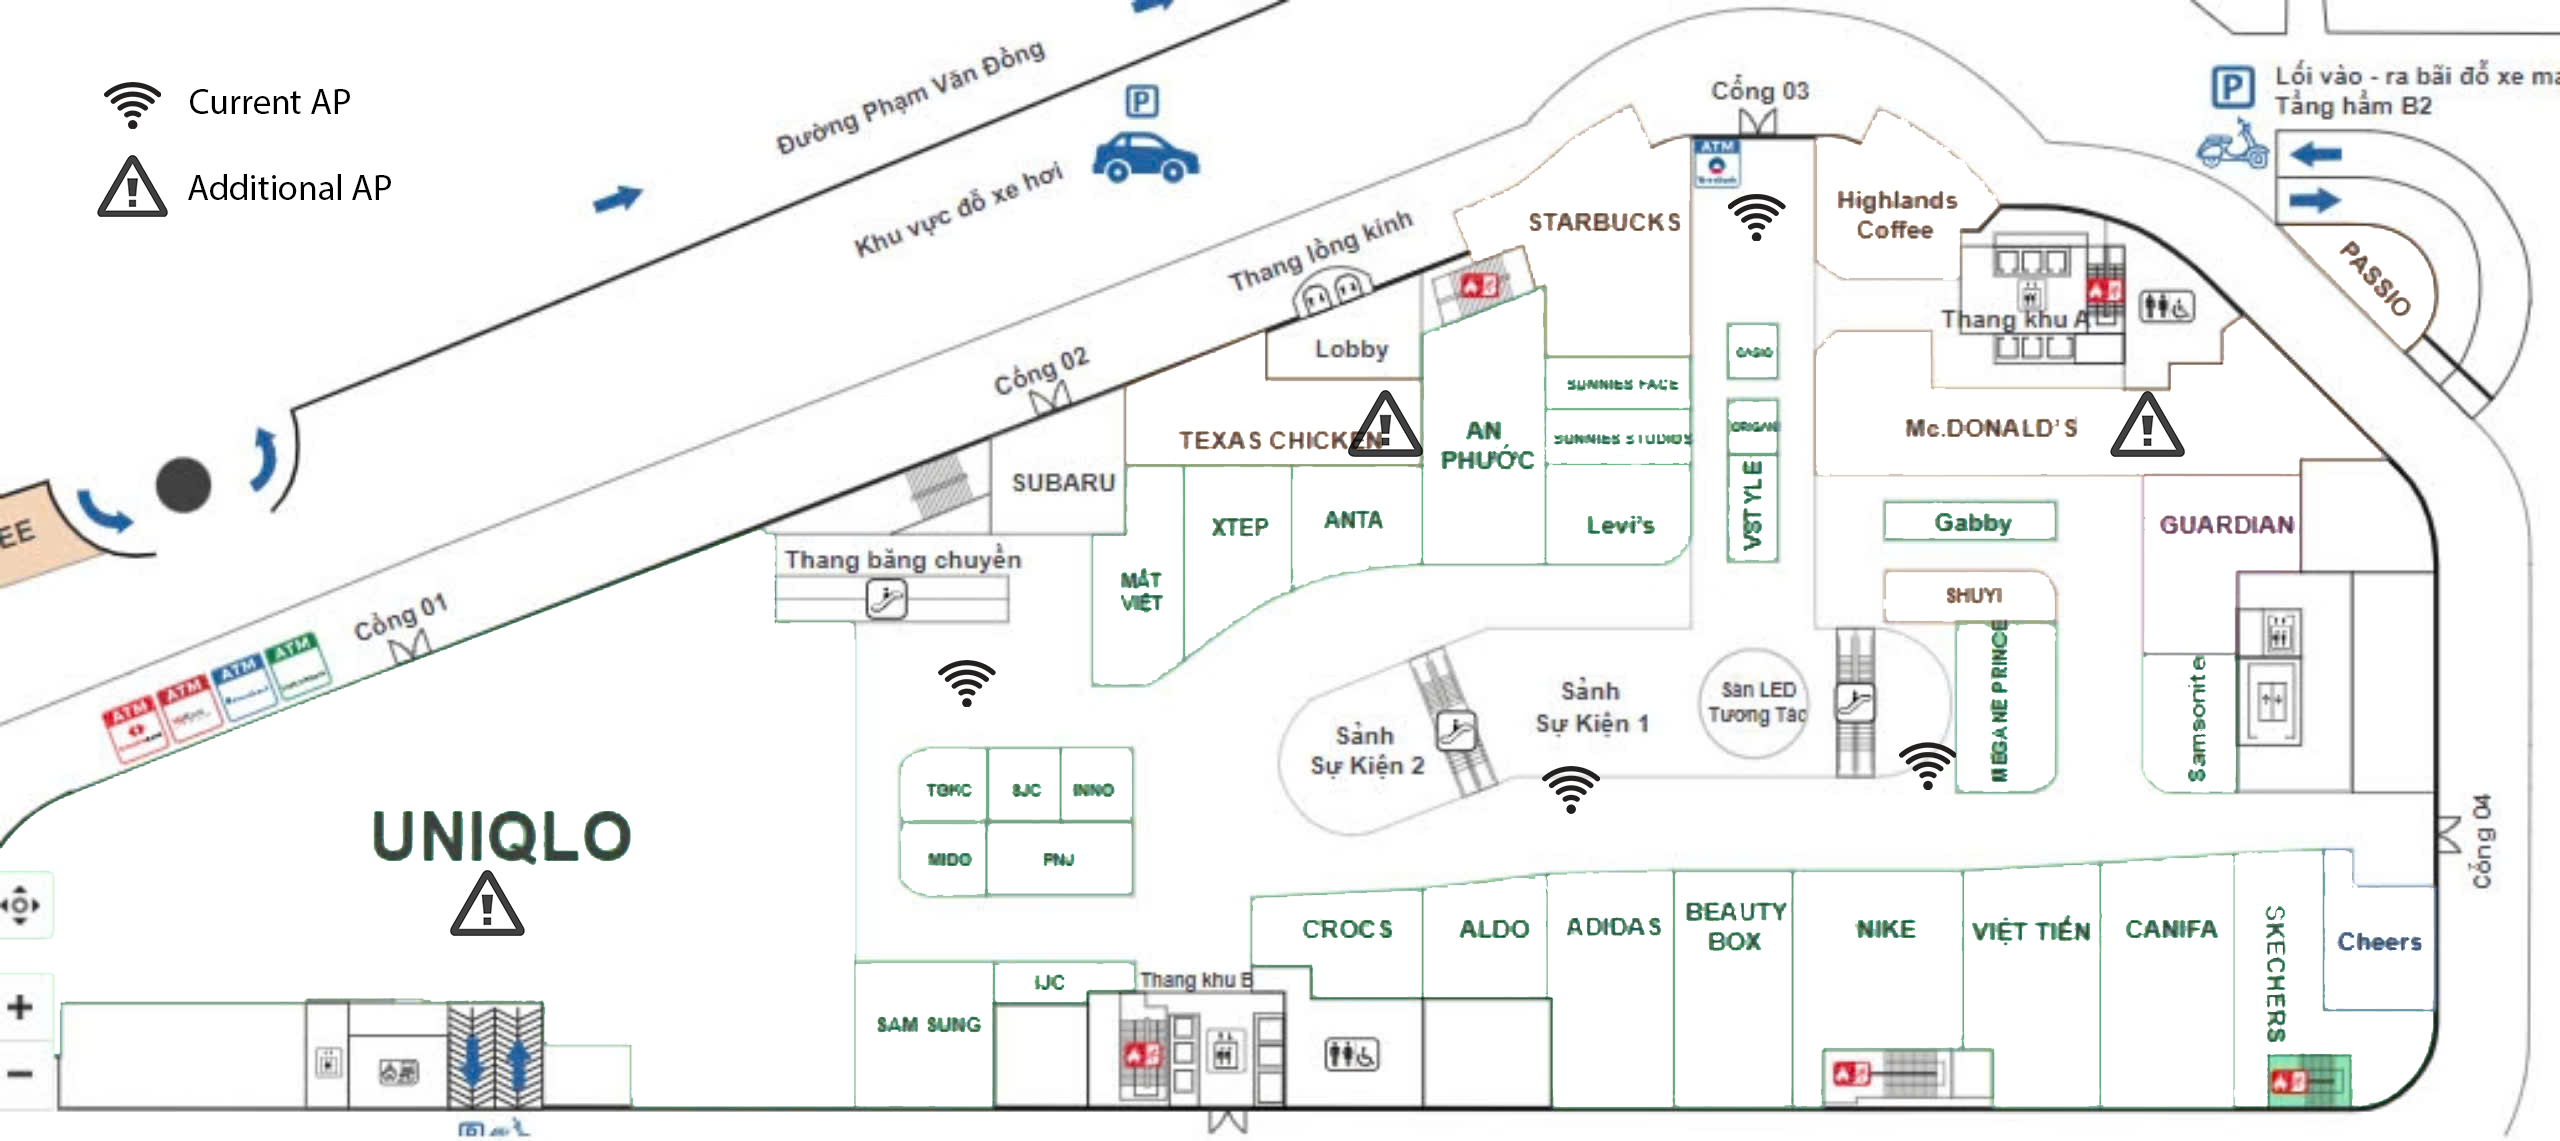
\includegraphics[width=0.48\textwidth]{fig6_acesspoint_suggestion.png}
    \caption{A proposed access point placement.}
\end{figure}

Furthermore, access points should be placed at higher elevations to improve signal distribution. By placing them at higher positions, signals are less likely to be obstructed. Additionally, mesh Wi-Fi networks that uses multiple nodes, could be explored to achieve full building coverage. However, it's important to note that this approach may lead to reduced speeds due to bandwidth division. These conclusions are drawn from the current survey and may require reassessment as the network evolves. Regular site surveys are recommended to monitor network performance and identify areas for optimization.

\section{Roaming Architecture}

This section will explain the meaning of roaming in wireless local area networks (WLANs), and introduce the basics of two types of roaming. It also describes the roaming model in the site survey.

\subsection{Definition of Roaming}

With one network, several access points must often be installed to cover a building adequately. [...] When a user moves between one cell - a floor of a building, let's say - and another, the system must provide for hand-off, so that users can roam the floors without dropping the connection. The access point must automatically start handling the user's data traffic and redirect messages sent to the old access point. Almost all wireless LAN products have software that enables users to roam between access points, once the software notices a diminishing signal, it searches the domain for the strongest access-point signal and connects to that \cite{wickelgren1996}.

Roaming in WLAN is categorised into two types: internal roaming (layer 2) and external roaming (layer 3) \cite{wiki_roaming}. The study only focuses on internal roaming since it is implemented in the area where the site survey was conducted.

\subsection{Internal Roaming}

Internal roaming or Layer 2 roaming  refers to roaming that occurs within the same subnet or distribution system. In this case, the device’s IP address remains unchanged, and the transition between APs is nearly seamless. Generally, the client device is not required to re-authenticate in internal roaming. The internal roaming process is shown in Fig. 7 and Fig. 8.

\begin{figure}[htbp]
    \centering
    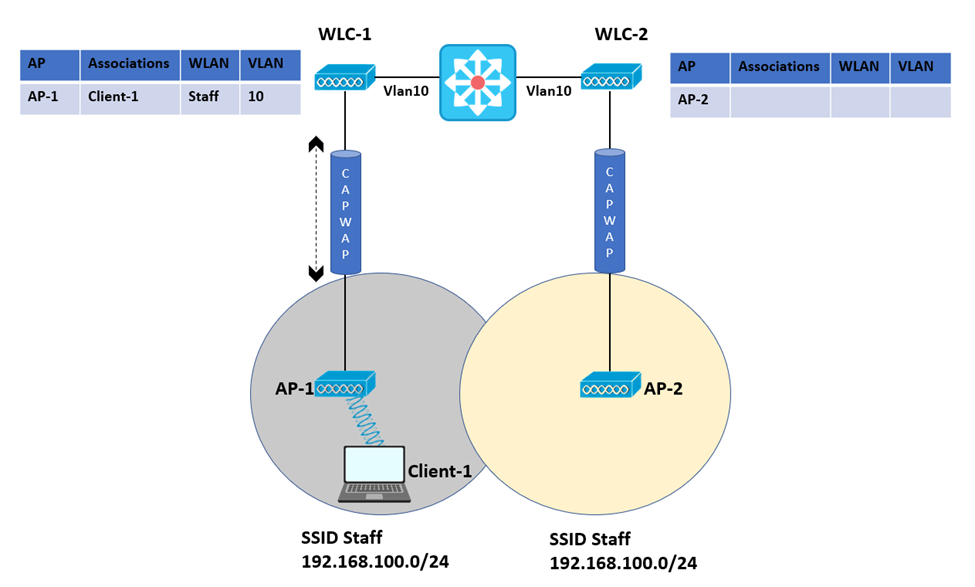
\includegraphics[width=0.46\textwidth]{fig7_internal_roaming.png}
    \caption{A picture displays the wireless local area network (WLAN) for internal roaming \cite{study_ccnp}.}
\end{figure}

Fig. 7 illustrates two WLAN controllers (WLCs), where WLC-1 contains a database entry for Client-1. The client moves to AP-2, roaming from one WLC to another. This handover, managed by both WLCs, involves the client’s IP address. Prior to the roam, the client is connected to AP-1, receiving an IP address based on the subnet and VLAN settings configured on WLC-1’s WLAN. Since the WLAN Staff is assigned to VLAN 10, the client uses an IP address from the 192.168.100.0/24 subnet range.

When the client connects to a new Access Point, it tries to retain its current IP address or requests a new one from the DHCP server. Fig. 8 shows the client moving to AP-2, where the WLAN Staff still operates on VLAN 10 with the same 192.168.100.0/24 subnet, the same as WLC-2.

\begin{figure}[htbp]
    \centering
    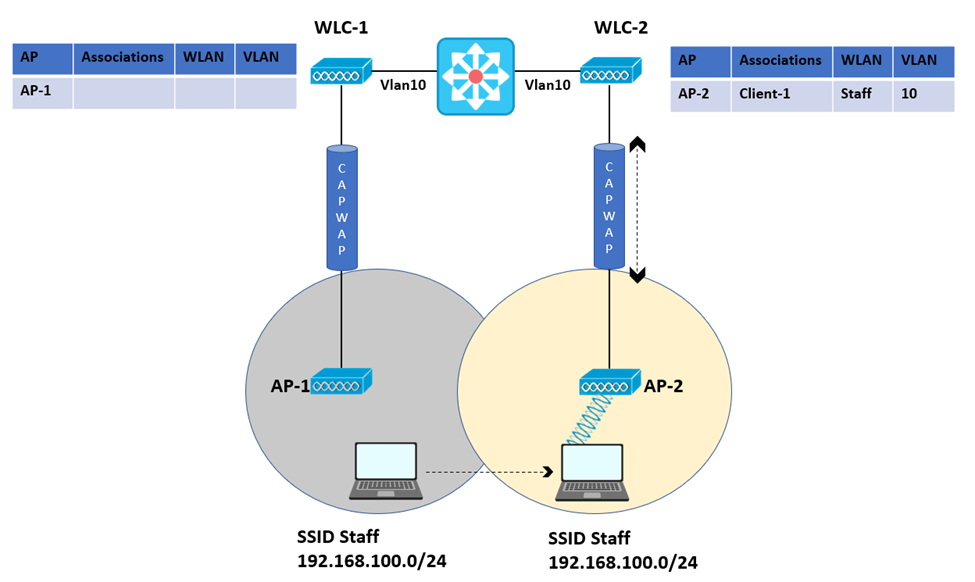
\includegraphics[width=0.46\textwidth]{fig8_internal_roaming_after_roaming.png}
    \caption{The internal roaming scenario showcasing the handover process between two WLCs \cite{study_ccnp}.}
\end{figure}

Although the client switched between different APs, it remained within the same subnet and VLAN, which qualifies as a Layer 2 intercontroller roam. This type of local-to-local roaming allows the client to keep its IP address, and the process is quick, typically taking less than 20 ms.

The example above illustrates the Layer 2 roaming process of a client. Delving deeper into the technical aspects, there are more procedures involved than simply finding a new AP to communicate with \cite{wlan_fundamentals}. 

(*) These tasks are not mandatory, as they are not explicitly defined in the 802.11 standard.

\begin{itemize}
    \item Client associates with the initial AP.
    \item Client roams to a new AP.
    \item Previous AP buffers data destined for the roaming client. (*) 
    \item New AP indicates to the previous AP that the client has successfully roamed. This is typically done via a unicast or multicast packet from the old AP to the new AP with the source MAC address set to the MAC of the roaming client. (*)
    \item After receiving confirmation, the previous AP should forward the buffered data to the new AP.
    \item It is crucial for the previous AP to recognize that the client has moved away from its coverage area. Previous AP updates its MAC address table to remove the roaming client.
    \item New AP needs to update MAC address tables on the infrastructure switches to add the roaming client.
\end{itemize}

To give an example of internal roaming, the GigaMall network in the site survey above employs internal roaming, as the SSID of the access points is the same—\#GigaMall - Swifi Free. The device's IP address remained unchanged when transitioning to another access point. As mentioned earlier, there were areas where the roaming process was seamless and others where connections were interrupted during the roaming process. Fig. 9 demonstrates how seamless roaming works in the site survey.

\begin{figure}[htbp]
    \centering
    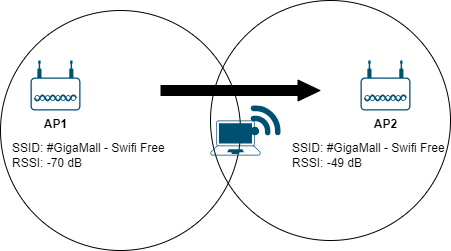
\includegraphics[width=0.48\textwidth]{fig9_seamless_roaming_work.png}
    \caption{An illustration of how seamless roaming works in the site survey.}

\end{figure}

\subsection{External Roaming}

External Roaming (also known as Layer 3 Roaming) is the process in which a device moves between different subnets when switching its connection from one AP to another. This type of roaming is more complex than internal roaming (Layer 2 Roaming), where the device only moves between APs within the same subnet without changing its IP address.

In a typical multi-floor buildings, application sessions are disrupted due to VLAN roaming. Mobile IP offers a standardized solution to address this issue by enabling seamless Layer 3 roaming across WLANs.This ensures uninterrupted connectivity for various applications \cite{wlan_fundamentals}. Fig. 10 and Fig. 11 below depicts the external roaming process.

\begin{figure}[htbp]
    \centering
    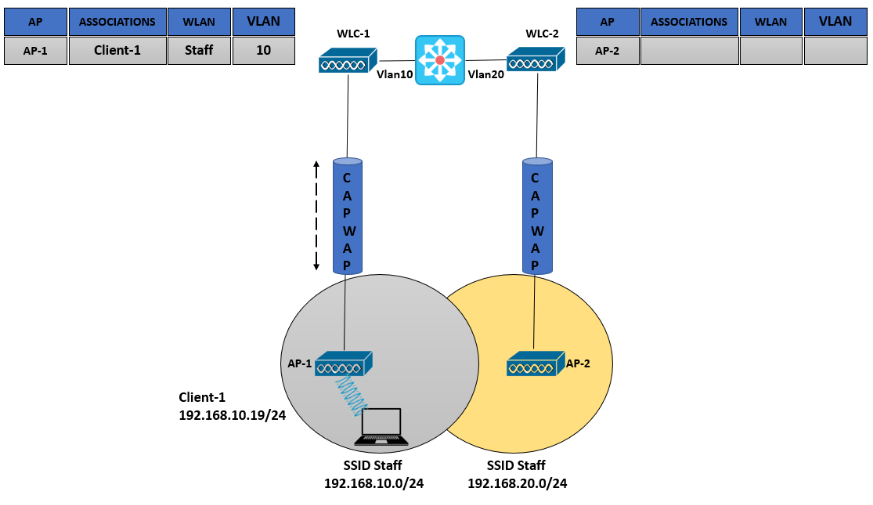
\includegraphics[width=0.5\textwidth]{fig10_external_roaming.png}
    \caption{A picture displays the WLAN environment for external roaming \cite{study_ccnp}.}
\end{figure}

WLAN interfaces on WLCs can be assigned to different VLANs and subnets. When a client switches between WLCs, it effectively roams between subnets. However, wireless clients typically remain unaware of subnet changes and only perceive AP roaming.

\begin{figure}[htbp]
    \centering
    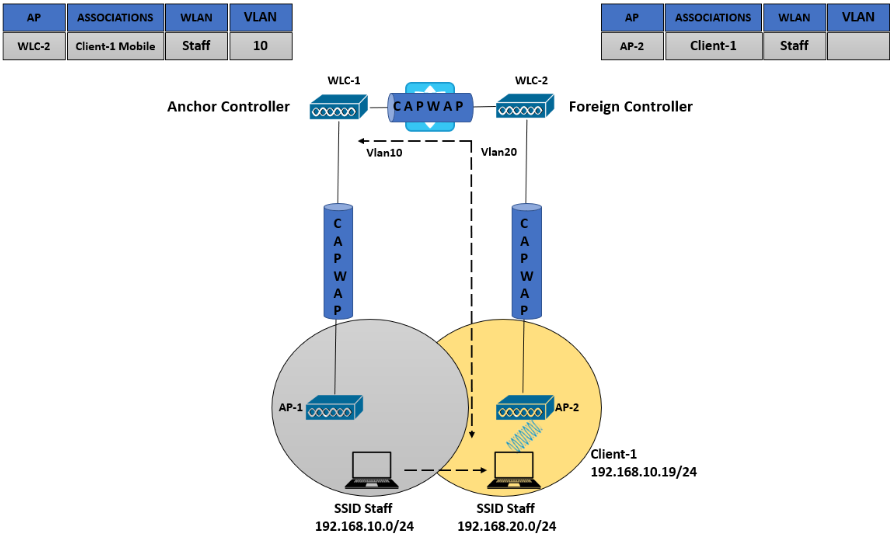
\includegraphics[width=0.5\textwidth]{fig11_external_roaming_after_roaming.png}
    \caption{A WLAN external roaming scenario showcasing the handover process between two WLCs \cite{study_ccnp}.}
\end{figure}

\section{Conclusion}

This study has identified weaknesses in the wireless network within the area through a comprehensive site survey and an analysis of the existing roaming architecture. It also emphasizes the critical role of site surveys. The data collected during the survey serves as a foundation for proposing enhancements to improve signal coverage and minimize interference, enabling the design of an efficient wireless network design to meet the needs of entertainment, social networking and uploading short videos and images.

Furthermore, the report provided a comprehensive overview of roaming, including its definition and classification. This knowledge is instrumental in understanding how to maintain seamless connectivity across various access points, thereby enhancing overall network performance and user experience within the academic environment.

\begin{thebibliography}{9}

\bibitem{wickelgren1996}
I. J. Wickelgren, "Local-area networks go wireless," \textit{IEEE Spectrum}, vol. 33, pp. 38--40, 1996.

\bibitem{wiki_roaming}
Wikipedia contributors, "Wireless LAN - Wikipedia," 2024. [Online]. Available: \url{https://en.wikipedia.org/wiki/Wireless_LAN#Roaming}. [Accessed: 5-Oct-2024].

\bibitem{study_ccnp}
Study CCNP, ``WLAN Intercontroller Layer 2 and Layer 3 Roaming,'' 2024. [Online]. Available: \url{https://study-ccnp.com/wlan-intercontroller-layer-2-layer-3-roaming}. [Accessed: 5-Oct-2024].

\bibitem{wlan_fundamentals}
P. Roshan and J. Leary, \textit{802.11 Wireless LAN Fundamentals}. Cisco Press, 2003.

\end{thebibliography}

\end{document}
